\documentclass[12pt,a4paper,oneside]{article} %hidelinks
\usepackage[english]{babel}
\usepackage{natbib}
\usepackage{url}
\usepackage[utf8x]{inputenc}
\usepackage[T1]{fontenc}
\usepackage{amsmath}
\usepackage{graphicx}
\graphicspath{{images/}}
\usepackage{parskip}
\usepackage{fancyhdr}
%\usepackage{vmargin}
\usepackage{subcaption}
\usepackage[table]{xcolor}												% habilita cores (capa)
\usepackage[some]{background} 									% papel de parede (capa)
\usepackage{indentfirst} 										% identacao dos paragrafos
\usepackage{hyperref} 
\usepackage{ucs}
\usepackage[top=3cm,bottom=3.5cm,right=2.5cm,left=2.5cm]{geometry} 

\usepackage{amsfonts}											% ferramentas matematicas
\usepackage{amssymb}											% ferramentas matematicas
\usepackage{pdfpages}
\usepackage{etoolbox}
\usepackage{sidecap}

\usepackage{listings}
\usepackage{color}

\definecolor{codegreen}{rgb}{0,0.6,0}
\definecolor{codegray}{rgb}{0.5,0.5,0.5}
\definecolor{codepurple}{rgb}{0.58,0,0.82}
\definecolor{backcolour}{rgb}{0.95,0.95,0.92}

\definecolor{mygreen}{rgb}{0,0.6,0}
\definecolor{mygray}{rgb}{0.5,0.5,0.5}
\definecolor{mymauve}{rgb}{0.58,0,0.82}

\lstdefinestyle{mystyle}{
    backgroundcolor=\color{backcolour},   
    commentstyle=\color{codegreen},
    keywordstyle=\color{black},
    numberstyle=\tiny\color{codegray},
    stringstyle=\color{codepurple},
    basicstyle=\ttfamily\small,
    breakatwhitespace=false,         
    breaklines=true,                 
    captionpos=b,                    
    keepspaces=true,                 
    numbers=none,                    
    numbersep=5pt,                  
    showspaces=false,                
    showstringspaces=false,
    showtabs=false,                  
    tabsize=2
}

\lstdefinestyle{textstyle}{
    backgroundcolor=\color{white},   
    commentstyle=\color{codegreen},
    keywordstyle=\color{magenta},
    numberstyle=\tiny\color{codegray},
    stringstyle=\color{codepurple},
    basicstyle=\footnotesize,
    breakatwhitespace=false,         
    breaklines=true,                 
    captionpos=b,                    
    keepspaces=true,                 
    numbers=none,                    
    numbersep=5pt,                  
    showspaces=false,                
    showstringspaces=false,
    showtabs=false,                  
    tabsize=2
}

\lstset{style=mystyle}

%\setmarginsrb{2.5 cm}{2.5 cm}{2.5 cm}{2.5 cm}{1 cm}{1.5 cm}{1 cm}{1.5 cm}

\definecolor{titlepagecolor}{cmyk}{.6,0,.9,.40} % definicao de cor

\backgroundsetup{
scale=1,
angle=0,
opacity=1,
contents={\begin{tikzpicture}[remember picture,overlay]
 \path [fill=titlepagecolor] (current page.west)rectangle (current page.north east); 
 \draw [color=white, very thick] (5,0)--(5,0.5\paperheight);
\end{tikzpicture}}
} % configura o plano de fundo

\makeatletter                   
\def\printauthor{%                  
    {\large \@author}}          
\makeatother

\title{RASv.2 Software Guide}								% Title
\date{7 June 2018}											% Date
\author{%
    \textbf{Eficent Business and IT Consulting Services S.L.}% \vspace{40pt}\\
    }

\pagestyle{fancy}
%\fancyhf{}
\rhead{Eficent Business and IT Consulting Services S.L.}
\lhead{RASv.2 Software Guide}
%\cfoot{\thepage}
\rfoot[]{\begin{picture}(10,10) \put(-40,-40){
\includegraphics[width=30mm]{images/eficent}} \end{picture}}
%\pagestyle{headings}
\begin{document}

%%%%%%%%%%%%%%%%%%%%%%%%%%%%%%%%%%%%%%%%%%%%%%%%%%%%%%%%%%%%%%%%%%%%%%%%%%%%%%%%%%%%%%%%%

\begin{titlepage}
	\BgThispage
	\newgeometry{left=1cm,right=6cm,bottom=2cm}
	\vspace*{0.4\textheight}
	\noindent
	\textcolor{white}{{\Huge\textbf{\textsf{RASv.2 Software Guide}}}\\ \vspace{15pt}\hspace{110pt} version one}
	\vspace*{2cm}\par
	\noindent
	\begin{minipage}{0.35\linewidth}
		\begin{flushright}
			\printauthor
		\end{flushright}
	\end{minipage} \hspace{15pt}
	%
	\begin{minipage}{0.04\linewidth}
		\textcolor{titlepagecolor}{\rule{2pt}{250pt}}
	\end{minipage} \hspace{20pt}
	%
	\begin{minipage}{0.8\linewidth}
		\vspace{5pt}
		%	  \begin{abstract} 
		This user guide serves as a reference for the initial configuration, functioning and frequently asked questions about the RAS v.2 and its software. 
		%	  \end{abstract}
	\end{minipage}
\end{titlepage}
\restoregeometry

%%%%%%%%%%%%%%%%%%%%%%%%%%%%%%%%%%%%%%%%%%%%%%%%%%%%%%%%%%%%%%%%%%%%%%%%%%%%%%%%%%%%%%%%%

\tableofcontents
%\pagebreak
%\listoffigures
\pagebreak

%%%%%%%%%%%%%%%%%%%%%%%%%%%%%%%%%%%%%%%%%%%%%%%%%%%%%%%%%%%%%%%%%%%%%%%%%%%%%%%%%%%%%%%%%

\section{General Overview}

The RFID Attendance System v2.0 or RAS v2.0 is a redesign of the RAS concept developed by \textbf{\href{http://www.eficent.com/about-us/}{Eficent Business and IT Consulting Services S.L.}} \citep{eficent}for the first version, taking only the main idea and a few components from it (concretely the \href{https://www.nxp.com/docs/en/data-sheet/MFRC522.pdf}{MFRC522} \citep{rfid} and the use of a buzzer); and upgrading several functional aspects like:

\begin{itemize}
	\item The device "brain" role is developed by the \href{https://www.raspberrypi.org/products/raspberry-pi-zero-w/}{Raspberry Pi Zero W} \citep{rpi} instead of the NodeMCU. While the second one can only run sequential code with a strictly defined structure (setup and loop), the first one gives total freedom for programming due to its nature as a "little computer".
	\item The user visual feedback, generated in this case using a \href{https://www.elecrow.com/download/SH1106\%20datasheet.pdf}{SH1106 OLED display} \citep{oled}, while at the RAS v1.0 it was created by means of two color LEDs.
	\item The parameters configuration is not integrated alongside the WiFi configuration anymore, because they are modified using a configuration portal through a web browser. It also means that they can be changed every time it is necessary.
\end{itemize}

There are also completely new features:

\begin{itemize}
	\item A user menu in the own device, which appears when it is turned on, and that offers several possibilities to the user, like the common RFID-Odoo functioning, a RFID reader functionality to be able to know the ID of a card/key, a reset for the WiFi parameters... This menu is navigated by means of two buttones located at the sides of the device: right side for going down in the menu, and left side to select an option (they are capacitive buttons, so they are not visible at first sight).
	\item The possibility of upgrading the software to newer versions or even change the compatible Odoo version if there is a change in yours company Odoo. It can be done by installing a new image in the RPi, or through \emph{pip}.
\end{itemize}

For now, the updating through \emph{pip} is not finished, so the update is carried out by pulling the last version of the code from a repository.


\section{RPi Zero W initial configuration}

The Raspberry Pi Zero W, like the rest of boards of the RPi family, works by means of a MicroSD card in which a suitable OS must be flashed or installed. 

\textbf{Eficent Business and IT Consulting Services S.L.} provides deployed images for the RAS v2.0 that when flahsed into the SD, allow a direct use of the device functionalities.

However, for this software guide, the complete process to configure a RPi Zero W from scratch to run the RAS v2.0 functionalities without employing the aforementioned image is explained.

Before starting, acknowledgements must be given to several free-software developers whose code has been used to create some functionalities or to control some devices. They are:

\begin{itemize}
	\item \href{https://github.com/jasbur/RaspiWiFi/tree/master}{Jason Burgett} $\rightarrow$ WiFi AP point functionality.
	\item \href{https://github.com/lthiery/SPI-Py}{Louis Thiery} $\rightarrow$ SPI protocol library.
	\item \href{https://github.com/mxgxw/MFRC522-python}{Mario Gómez} $\rightarrow$ MFRC522 control library. 
	\item \href{https://github.com/rm-hull/luma.examples}{Richard Hull} $\rightarrow$ OLED display control library.
\end{itemize}

The following steps have been used and tested in Ubuntu 16.04. To configure the WiFi, for Mac, it can be interesting to follow \href{https://desertbot.io/blog/setup-pi-zero-w-headless-wifi}{Setup Pi Zero W Headless WiFi} \citep{mac} alongside our guide. For Windows, you can consult \href{https://core-electronics.com.au/tutorials/raspberry-pi-zerow-headless-wifi-setup.html}{How To Setup Raspberry Pi Zero W Headless WiFi} \citep{windows}.

\subsection{RPi General Configuration}

\begin{enumerate}
	\item Download the Raspbian Lite image from the \href{https://www.raspberrypi.org/downloads/raspbian/}{Raspberry official site} \citep{rasp-off} as a ZIP.
	\item Download \href{https://etcher.io/}{Etcher} \citep{etcher} to flash the SD card.
	\item Insert the SD card in the PC.
	\item Execute Etcher. Once it is opened, select the Raspbian Lite image, select the SD card as drive and click in "Flash!". It will take several minutes.
	\item Once the SD card has been flashed, go to the two generated partitions (boot and rootfs), in terminal or using the filesystem (folders).
	\item To enable the \textbf{ssh} (we will use it to connect to the RPi), create a blank file called "ssh" (no extension needed) at the boot partition (not the boot folder of the rootfs partition).
	\item Go to the rootfs partition and open the file $etc/wpa\_supplicant/wpa\_supplicant.conf$ (beware and be sure you are not at your computer folders, you have to modify the SD ones!).
	\item Add the following lines to the end (substituting the contents into the ):
	\begin{lstlisting}[language=sh,style=textstyle]
	
		network={
  			ssid="my network name"
  			psk="my network password"
		}
	\end{lstlisting}
	\emph{\textbf{*}For other possible network configurations, see \href{https://www.raspberrypi.org/documentation/configuration/wireless/wireless-cli.md}{Setting up WiFi via the command line}}.
	\linebreak\linebreak\linebreak
	\item Add the \href{http://www.nationsonline.org/oneworld/country_code_list.htm}{country code} too (to choose the correct frequency bands), as follows (use the ISO ALPHA-2 Code, that is, the one which employs two letters):
	\begin{lstlisting}[language=sh,style=textstyle]
	
		country=XX
	\end{lstlisting}
    \item Go to $etc/network/$ and open the \textit{interfaces} file.
    \item Find this block in the file (if it is not present, go to the next step):
    \begin{lstlisting}[language=sh,style=textstyle]
	
		allow-hotplug wlan0
        iface wlan0 inet manual
            wpa-conf /etc/wpa_supplicant/wpa_supplicant.conf
	\end{lstlisting}
	\item Substitute the block with (if it is not present, just add the next block to the end of the file):
	\begin{lstlisting}[language=sh,style=textstyle]
	
		auto wlan0
        allow-hotplug wlan0
        iface wlan0 inet dhcp
            wpa-conf /etc/wpa_supplicant/wpa_supplicant.conf
	\end{lstlisting}
	\emph{\textbf{*}There is the possibility of fixing the Raspberry Pi Zero W IP address (static) so it is easier to find. See \href{https://medium.com/@DavidMaitland/raspberry-pi-zero-headless-setup-92fb72daf88d}{David Maitland Raspberry Pi Zero Headless Setup}} for more details.
	\item Unmount the partitions and eject the SD card.
	\item Introduce it in the RPi Zero, plug the cable to give it power and wait for some time so that the RPi can configure itself.
	\item Open a terminal in your computer to connect through SSH to the RPi. There are several ways (from quick (maybe some are more difficult) to slow but easier):
	\begin{enumerate}
		\item Try the next command:
		\begin{lstlisting}[language=sh]
	
			ssh pi@raspberrypi.local
		\end{lstlisting}
		If it worked, it will ask you for a password. Introduce "raspberry" (default password), and you will be able to manage the RPi through terminal by SSH. Go to step 17 now.
		
		\emph{\textbf{*}If you have another RPi connected or you had in the past, it may not work. To clear any previous reference to \textit{raspberry.local}, use:}
		\begin{lstlisting}[language=sh]
	
			ssh-keygen -R raspberrypi.local
		\end{lstlisting}
		\item If the previous method didn't worked, we need to find the RPi IP adress. To do that, there are two possibilities:
		\begin{enumerate}
			\item Use \emph{nmap}:
			\begin{lstlisting}[language=sh]
	
				sudo apt-get install nmap
				
				nmap -sn 192.168.1.0/24
			\end{lstlisting}
			It will show all the connected devices to the WiFi network by their IPs. The problem is that you won't know which one matches your RPi. You will need to try until you find them, or use the command before connecting the RPi, so that the IP that appears when it is connected would be the right one.
			\item Download a smartphone app called Fing. Once it is installed, when you initialize it, it will look for the connected devices to the same network than it, and it will tell you the device description. Look for \textbf{Raspberry Pi}.
		\end{enumerate}
		\item Once we know the RPi IP adress, use the next command with the proper IP:
		\begin{lstlisting}[language=sh]
	
			ssh pi@192.168.1.XX
		\end{lstlisting}
		
		If it worked, it will ask you for a password. Introduce "raspberry" (default password), and you will be able to manage the RPi through terminal by SSH. Go to step 17 now.
	\end{enumerate}
	\item Now, let's configure the RPi for our use. Introduce the following command to opne the configuration page:
	\begin{lstlisting}[language=sh]
	
		sudo raspi-config
	\end{lstlisting}
	\item Use the \textit{\textbf{Change User Password}} option, and set your own password.
	\item Use the \textit{\textbf{Advanced Options}} to \textit{\textbf{Extend Filesystem}}.
	\item At \textit{\textbf{Interfacing Options}}, enable SPI and I2C.
	\item Then, go to \\textit{textbf{Finish}} in the main page and reboot.
	\item  When the RPi SSH connections comes back to be possible, log in using your new password.
	
	\emph{\textbf{*}To save energy and speed up the device (optional settings):}
	\begin{itemize}
		\item Boot up into multi-user mode (disabling the GUI on boot):
		\begin{lstlisting}[language=sh]
	
			sudo systemctl set-default multi-user.target
		\end{lstlisting}
		\item To disable the HDMI, edit \textit{/etc/rc.local} and add (above \textit{exit 0}):
		\begin{lstlisting}[language=sh,style=textstyle]
	
		/usr/bin/tvservice -o
		\end{lstlisting}
	\end{itemize}
	\item Update and upgrade:
	\begin{lstlisting}[language=sh]
	
		sudo apt-get -y update
		
		sudo apt-get -y upgrade
	\end{lstlisting}
	\item Check if the SPI is really enabled using:
	\begin{lstlisting}[language=sh]
	
		ls -l /dev/spidev*
	\end{lstlisting}
	
	You must see two devices, one for each SPI bus.
	\item Use the following commands to install some additional packages for the I2C:
	\begin{lstlisting}[language=sh]
	
		sudo apt-get install -y python-smbus
		
		sudo apt-get install -y i2c-tools
	\end{lstlisting}
	\item Check the I2C using:
	\begin{lstlisting}[language=sh]
	
		ls -l /dev/i2c*
	\end{lstlisting}
	\item Install important programs/packages:
	\begin{lstlisting}[language=sh]
	
		sudo apt-get install git
		
		sudo apt-get install python-dev -y
	\end{lstlisting}
\end{enumerate}
\pagebreak

\subsection{WiFi AP mode configuration}

\begin{enumerate}
	\item Clone the repository and enter the folder:
	\begin{lstlisting}[language=sh]
	
		cd
		
		git clone https://github.com/jasbur/RaspiWiFi.git
		
		cd Raspiwifi
	\end{lstlisting}
	\item Run the next command (the installation will take several minutes):
	\begin{lstlisting}[language=sh]
	
		sudo python3 initial_setup.py
	\end{lstlisting}
	
	This script will install all necessary prerequisites, copy configuration files, and reboot. When it finishes booting it should present itself in \textit{Configuration Mode} as a WiFi access point with the name \textit{RaspiWiFi Setup XXXX} (the XXXX is a number that depends on the Raspberry, and it is unique for each one of them).
	\item To enter again the RPi (these following steps are also useful for the normal use of the WiFi AP mode):
	\begin{itemize}
		\item Connect to the \textit{RaspiWiFi Setup XXXX} access point using any other WiFi enabled device.
		\item Navigate to \textbf{http://10.0.0.1:9191} using any web browser on the device you connected with.
		\item Select the WiFi connection you'd like your Raspberry Pi to connect to from the drop down list and enter its wireless password on the page provided. If no encryption is enabled, leave the password box blank.
		\item Click the \textit{Connect} button.
		\item At this point your Raspberry Pi will reboot and connect to the access point specified.
	\end{itemize}
	\item Finally, enter the RPi again using SSH as it was explained before.
\end{enumerate}

\subsection{SPI and MFRC522 configuration}

\begin{enumerate}
	\item Clone the following repository and enter its folder:
	\begin{lstlisting}[language=sh]
	
		cd
		
		git clone https://github.com/lthiery/SPI-Py.git
		
		cd SPI-py
	\end{lstlisting}
	\item Install the SPI module necessary for the MFRC522 library:
	\begin{lstlisting}[language=sh]
	
		sudo python setup.py install
	\end{lstlisting}
	\item Then, clone the MFRC522 repository and enter its folder:
	\begin{lstlisting}[language=sh]
	
		cd
		
		git clone https://github.com/mxgxw/MFRC522-python.git
		
		cd MFRC522-python
	\end{lstlisting}
	\item Connect the RFID Reader to the RPi Zero GPIO pins. The template for the explanation is: \textbf{\emph{RPI-GPIO-pin:RFIDReader-pin}}. Concretely (I will refer here to the physical position of the GPIO pins, it can be found at \href{https://pinout.xyz/pinout/io_pi_zero#}{RPi Zero W Pinout}).
	\setlength{\arrayrulewidth}{0.8mm}
	\begin{table}[h]
	\centering
	\rowcolors{2}{green!80!yellow!50}{green!70!yellow!40}
	\begin{tabular}{| c | c |}
		\hline
		\textbf{GPIO (BOARD)} & \textbf{RFID pin} \\ \hline
		$GPIO 17$ & 3.3V \\ \hline
		$GPIO 19$ & MOSI \\ \hline
		$GPIO 20$ & GND \\ \hline
		$GPIO 21$ & MISO \\ \hline
		$GPIO 22$ & RST \\ \hline
		$GPIO 23$ & SCK \\ \hline
		$GPIO 24$ & SDA \\ \hline
	\end{tabular}
	\caption{GPIO (RPi) - RFID pins convsersion table}
	\label{gpio}
	\end{table}
	\item Make a test to check that the installation has been succesful:
	\begin{lstlisting}[language=sh]
	
		python Read.py
	\end{lstlisting}
	Pass a card next to the RFID card, and it should be written at the terminal.
\end{enumerate}

\pagebreak

\subsection{SH1106 OLED screen configuration}

\begin{enumerate}
	\item Install some necessary packages:
	\begin{lstlisting}[language=sh]
	
		cd
		
		sudo apt-get install python-dev python-pip libfreetype6-dev libjpeg-dev build-essential
	\end{lstlisting}
	\item Install the \href{https://luma-oled.readthedocs.io/en/latest/}{luma.oled} package (it will take several minutes):
	\begin{lstlisting}[language=sh]
	
		sudo -H pip install --upgrade luma.oled
	\end{lstlisting}
	\item Wire up the display to the RPi (same explanation template than for the MFRC522):
	\setlength{\arrayrulewidth}{0.8mm}
	\begin{table}[h]
	\centering
	\rowcolors{2}{green!80!yellow!50}{green!70!yellow!40}
	\begin{tabular}{| c | c |}
		\hline
		\textbf{GPIO (BOARD)} & \textbf{OLED pin} \\ \hline
		$GPIO 1$ & VDD \\ \hline
		$GPIO 3$ & SDA \\ \hline
		$GPIO 5$ & SCK \\ \hline
		$GPIO 6$ & GND \\ \hline
	\end{tabular}
	\caption{GPIO (RPi) - SH1106 OLED display pins convsersion table}
	\label{gpio-oled}
	\end{table}
	\item Execute the following commands to confugire the user rights and install some necessary packages:
	\begin{lstlisting}[language=sh]
	
		sudo usermod -a -G i2c,spi,gpio pi
		
		sudo apt install python-dev python-pip libfreetype6-dev libjpeg-dev build-essential
		
		sudo apt install libsdl-dev libportmidi-dev libsdl-ttf2.0-dev libsdl-mixer1.2-dev libsdl-image1.2-dev
	\end{lstlisting}
	\item Reboot (\textit{sudo reboot}) and enter again the RPi through SSH.
	\item Clone the repository and enter its folder:
	\begin{lstlisting}[language=sh]
	
		cd
		
		git clone https://github.com/rm-hull/luma.examples.git
	\end{lstlisting}
	\item Install the luma libraries using (it will take several minutes):
	\begin{lstlisting}[language=sh]
	
		sudo -H pip install -e .
	\end{lstlisting}
	\item To test that everything is properly installed, run one of the \href{https://github.com/rm-hull/luma.examples}{examples}:
	\begin{lstlisting}[language=sh]
	
		cd examples
		
		python pi_logo.py -d sh1106
	\end{lstlisting}
	
	If the Raspberry Pi logo is displayed at the screen properly, the installation was succesful.
	\item To make the SH1106 the default display (now, the default one is the SSD1306), let's edit one of the luma.core files:
	\begin{lstlisting}[language=sh]
	
		sudo nano /usr/local/lib/python2.7/dist-packages/luma/core/cmdline.py
	\end{lstlisting}
	
	Go to the $create\_parser(description)$ method, and change the following line:
	\begin{lstlisting}[language=sh,style = textstyle]
	
		general_group.add_argument('--display', '-d', type=str, default=display_choices[0], help='Display type, supports real devices or emulators. Allowed values are: {0}'.format(', '.join(display_choices)), choices=display_choices, metavar='')
	\end{lstlisting}
	
	By:
	\begin{lstlisting}[language=sh,style = textstyle]
	
		 general_group.add_argument('--display', '-d', type=str, default=display_choices[6], help='Display type, supports real devices or emulators. Allowed values are: {0}'.format(', '.join(display_choices)), choices=display_choices, metavar='')
	\end{lstlisting}
	
	 So that the default field is loaded with the 6th element of the $display\_choices$ list (SH1106) instead of the 0th (SSD1306).
	 \item Finally, test again the screen functioning but using:
	 \begin{lstlisting}[language=sh]
	
		python pi_logo.py
	\end{lstlisting}
	
	If the Raspberry Pi logo is displayed at the screen properly, this final configuration was succesful.
\end{enumerate}

\subsection{RFID - OLED - ODOO and Configuration Server program configuration}

\begin{enumerate}
	\item Clone the repository:
	\begin{lstlisting}[language=sh]
	
		cd
		
		git clone https://github.com/lurobe94/Raspberry_Code.git
	\end{lstlisting}
	\item Install \href{http://flask.pocoo.org/}{Flask} and \href{https://pythonhosted.org/Flask-Babel/}{Flask-Babel} for the server:
	\begin{lstlisting}[language=sh]
	
		pip install Flask
		
		easy_install Flask-Babel
	\end{lstlisting}
	\item Test the server to create the \textbf{\textit{data.json}} file, which the main program will read to get the Odoo parameters:
	\begin{lstlisting}[language=sh]
	
		cd Raspberry_Code/Config-Portal/
		
		sudo python config-server.py
	\end{lstlisting}
	
	Enter using any web browser to the Raspberry IP address (192.168.1.XX) (it may change depending on the country), and the login portal will appear. Enter the credentials (they can be changed in hello-template.py) and the configuration portal will appear. Enter then the Odoo parameters, a RFID card ID for the administrator, and do not select the update option, as you just clone it.
	
	The data.json file must have been generated in the repository. Check the parameters are right.
	\item Test the main program by:
	\begin{lstlisting}[language=sh]
	
		python launcher.py
	\end{lstlisting}
	
	The program should work as expected. You can use the administrator RFID card to end the program.
	\item To configure the RPi to run the program at boot, edit the \textit{rc.local} file:
	\begin{lstlisting}[language=sh]
	
		sudo nano /etc/rc.local 
	\end{lstlisting}
	
	First, add these lines below the line "By default this script does nothing", to generate a log file for debugging errors.
	\begin{lstlisting}[language=sh,style = textstyle]
	
		exec 2> /tmp/rc.local.log  
    exec 1>&2                  
    set -x  
	\end{lstlisting}
	
	Add at the end, but before the \textbf{\textit{exit 0}} line, the following: 
	\begin{lstlisting}[language=sh,style = textstyle]
	
		python /home/pi/Raspberry_Code/launcher.py & 
    pyhton /home/pi/Raspberry_Code/Config-Portal/config-server.py & 
	\end{lstlisting}
	
	 Check the path, it can be different if you structured the folders in another way. Don't forget the \&, so that the programs runs in separated processes and the RPi can initialize itself without problems.
\end{enumerate}

\subsection{Final test}

\begin{enumerate}
	\item To test that everything is properly configured, use the following commands:
	\begin{lstlisting}[language=sh]
	
		rm -f data.json
	
		cd
		
		python Raspberry_Code/manual_reset.py
	\end{lstlisting}
	So that the data.json is deleted (and you can test the whole functioning of the device) and the Raspberry is rebooted, as well as the WiFi parameters are erased.
In this way, you must see first the screen that tells you to enter to the WiFi network, and that once you configure the WiFi, the program asks you to go to the configuration portal, and once you enter the parameters, the main program is executed properly.
\end{enumerate}

\section{Software operation processes}

In this section, the different functionalities of the main program, with all its subcomponents, and the configuration server are explained, as well as the possible feedback the user can receive, his/her interaction with the device... A diagram showing these functionalities and relations is presented in Figure \ref{sch-gen}.

\begin{figure}[h]
	\centering
	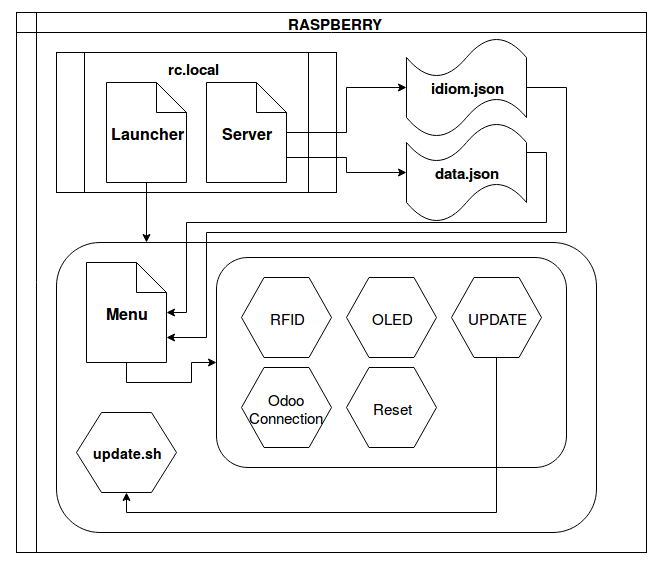
\includegraphics[width=0.7\textwidth]{images/scheme_general.png}
	\caption[General functioning scheme]{General functioning scheme}
	\label{sch-gen}
\end{figure}

The Raspberry Pi Zero W file \textbf{rc.local} allows to run all the commands written on it at boot, so two programs are called from there: the launcher of the main program (or RFID-OLED-Odoo program) and the configuration portal.

Both programs communicate using a text file known as \textbf{data.json}. It stores the parameters introduced using the configuration site, and they are read from this file by the main program. There is other shared file, \textbf{idiom.json}, which stores the language defined by the user from the displayed options.

Regarding the launcher, it first runs the program which executes the main functionalities, which are the RFID reading, the OLED siplay control, the connection with Odoo, the RAS v2.0 menu, the reset of the parameters, the update of the software...

If the update option is used at this main program, before exiting, the launcher will update the local repository with the last version of the code, and reboot the RPi.

The configuration portal uses another file called \textbf{credentials.json}, where the user and password of the configuration portal are stored.

\subsection{RFID-OLED-Odoo program}

\lstset{ %
  backgroundcolor=\color{backcolour},   % choose the background color
  basicstyle=\footnotesize,        % size of fonts used for the code
  breaklines=true,                 % automatic line breaking only at whitespace
  breakatwhitespace=false, 
  captionpos=b,                    % sets the caption-position to bottom
  commentstyle=\color{mygreen},    % comment style
  escapeinside={\%*}{*)},          % if you want to add LaTeX within your code
  keywordstyle=\color{blue},       % keyword style
  keepspaces=true,
  stringstyle=\color{mymauve},     % string literal style
}

This piece of software acts as the main program, running all the processes except the configuration server. It controls the OLED display, the MFRC522, the communication with Odoo..., as well as it allows user interface interaction due to its menu.

To understand it, let's review the different functions that conform it:

\subsubsection*{Libraries, global variables initialization and hardware configuration}

The first two included libraries are necessary to be capable of using the RPi GPIOs and the MFRC522 RFID reader. Then, the next three are employed for the connection to Odoo, as well as the following one is utilized for the WiFi checkings. Finally, the last libraries have different uses through the program, so their specific usage will be explained later. 

\begin{lstlisting}[language=python]
	
	#!/usr/bin/env python
	# -*- coding: utf-8 -*-

	import RPi.GPIO as GPIO
	import MFRC522

	import xmlrpclib
	import socket
	import urlparse

	try:
    	import httplib
	except:
    	import http.client as httplib

	import binascii
	import random
	import os, sys, time
	
\end{lstlisting}

Then, the OLED display management libraries are included, as well as another one for being able to read and write \emph{.json} files.

\begin{lstlisting}[language=python]

	from demo_opts import get_device
	from luma.core.render import canvas
	from PIL import ImageFont
	from PIL import Image
	from datetime import datetime

	import json

\end{lstlisting}

Some of the global variables are initialized here. Their meaninng will be clarified later, while explaining their role at the different functions.

\begin{lstlisting}[language=python]

	error = False
	card_found = False

	cnt_found = 0

	turn_off = False
	adm = True
	elapsed_time=0.0
	pos = 0
	enter = False
	reset = False
	on_Down = False
	on_OK = False

\end{lstlisting}

The GPIOs to manage the buttons are defined and configured in BOARD mode, so that the number of the pin is the physical position it has at the pinout.

\begin{lstlisting}[language=python]

	GPIO.setmode(GPIO.BOARD)  # Set's GPIO pins to BOARD GPIO numbering
	
	INPUT_PIN_DOWN = 31           # Pin for the DOWN button
	GPIO.setup(INPUT_PIN_DOWN, GPIO.IN)  # Set our input pin to be an input
	
	INPUT_PIN_OK = 29           # Pin for the OK button
	GPIO.setup(INPUT_PIN_OK, GPIO.IN)  # Set our input pin to be an input

\end{lstlisting}

Several dictionaries are defined, mostly to have all the displayed messages in the same format:

\begin{itemize}
	\item The first two dictionaries are the ones storing the messages for the normal functioning of the RFID - Odoo functionality, one for Spanish and other for English. The format of the stored data is: \emph{\textbf{key: [message, x position of the first line, number of lines, x position for the second line, x position of the third line, letter size]}}.
	
	The x position of the line is referred to the location of the sentence at the OLED display, regarding the \textit{x} coordinate.
	\item The next two dictionaries store the messages for the error situations, one for Spanish and other for English. The template is: \emph{\textbf{key: [number of messages, first message, number of lines (1),x position for the first line (1), x position for the second line (1), x position of the third line (1), second message, number of lines (2),x position for the first line (2), x position for the second line (2), x position of the third line (2), ...,  letter size]}}.
	
	The dotted line implies that more than two messages are possible.
	\item The following two dictionaries generate a bigger dictionary for each one of the two types of previous dictionaries (normal functioning or error). Like this, the language can be accessed using a variable.
	\item The last dictionary is employed to set the timezone for the time showed at the display.
\end{itemize}

\begin{lstlisting}[language=python]

	dic_en={' ': [" ",0,1,0,0,24], 'check_in': ['CHECKED IN',6,1,0,0,22],...}
	dic_es={' ': [" ",0,1,0,0,24], 'check_in': ['ENTRADA REGISTRADA',20,2,3,0,22],...}
	
	dicerror_en = {' ': [1," ",1,0,0,0,24], 'error1': [2,'Odoo communication failed',3,41,5,40,'Check the parameters',3,41,53,20,19],...}
	dicerror_es = {' ': [1," ",1,0,0,0,24], 'error1': [2,'Error de comunicacion',3,47,54,15,'Chequea los parametros',3,28,50,20,19],...}
	
	dic = {'es': dic_es, 'en': dic_en}
	dicerror = {'es': dicerror_es, 'en': dicerror_en}
	
	tz_dic = {'-12:00': "Pacific/Kwajalein",  '-11:00': "Pacific/Samoa",...}

\end{lstlisting}

The MFRC522 class is initialized, creating an instance to work with the device. Moreover, another dictionary is created, but this one is employed to select the functionalities from the menu. In this case, the parameter for each key is the name of a function.

\begin{lstlisting}[language=python]

	MIFAREReader = MFRC522.MFRC522()
	
	ops = {'0': rfid_hr_attendance, '1': rfid_reader, '2': settings, '3': back, '4': reset_settings, '5': change_language}

\end{lstlisting}

\subsubsection*{Starting function}

First, let's show the complete function:

\begin{lstlisting}[language=python]

	def m_functionality():
	    global device, lang
	    global update
	    global reset
	    global host, port, user_name, user_password, dbname
	    global admin_id, https_on
	    try:
	        device = get_device()
	        img_path = 		os.path.abspath(os.path.join(os.path.dirname(
	        __file__),'images', 'ef5.png'))
	        logo = Image.open(img_path).convert("RGBA")
	        fff = Image.new(logo.mode, logo.size, (0,) * 4)
	
	        background = Image.new("RGBA", device.size, "black")
	        posn = ((device.width - logo.width) // 2, 0)
	
	        img = Image.composite(logo, fff, logo)
	        background.paste(img, posn)
	        device.display(background.convert(device.mode))
	
	        json_file = open('/home/pi/Raspberry_Code/idiom.json')
	        json_data = json.load(json_file)
	        json_file.close()
	        lang = json_data["language"][0]
	        print lang
	        print json_data["language"]
	        lang2 = json_data["language"]
	        if lang2 == "es":
	            lang = "es"
	        else:
	            if lang2 == "en":
	                lang = "en"
	
	        time.sleep(4)
	        welcome_msg(device,17)
	        time.sleep(4)
	        if have_internet():
	            while not os.path.isfile("/home/pi/Raspberry_Code/data.json"):
	                screen_drawing(device,"config1")
	                time.sleep(2)
	                screen_drawing(device,"config2")
	                time.sleep(2)
	            if os.path.isfile("/home/pi/Raspberry_Code/data.json"):
	                json_file = open('/home/pi/Raspberry_Code/data.json')
	                json_data = json.load(json_file)
	                json_file.close()
	                host = json_data["odoo_host"][0]
	                port = json_data["odoo_port"][0]
	                user_name = json_data["user_name"][0]
	                user_password = json_data["user_password"][0]
	                dbname = json_data["db"][0]
	                admin_id = json_data["admin_id"][0]
	                timezone = json_data["timezone"][0]
	                os.environ['TZ'] = tz_dic[timezone]
	                time.tzset()
	                print time.strftime('%X %x %Z')
	                if "https" not in json_data:
	                    https_on = False
	                else:
	                    https_on = True
	
	                if "update" not in json_data:
	
	                    update = False
	                else:
	                    update = True
	                print "THIS IS UPDATE: " + str(update)
	            else:
	                raise ValueError("It is not a file!")
	        main()
	        if update == True:
	            screen_drawing(device,"update")
	            time.sleep(2)
	            screen_drawing(device," ")
	            GPIO.cleanup()
	        screen_drawing(device,"Bye!")
	        time.sleep(3)
	        screen_drawing(device," ")
	        GPIO.cleanup()
	        if reset == True:
	            screen_drawing(device," ")
	            reset_lib.reset_to_host_mode()
	        return update
	
	    except KeyboardInterrupt:
	        GPIO.cleanup()
	        pass


\end{lstlisting}

First, some global variables are included so that they can be used inside the function.

To briefly describe them: 

\begin{itemize}
	\item \emph{device}: it is necessary to create an instance of the display in the luma library.
	\item \emph{lang}: used to define the actual language.
	\item \emph{update}: it shows if the update option has been selected or not.
	\item \emph{reset}: idem, but for resetting the WiFi parameters.
	\item \emph{admin\_id}: idem, but for the detection of the administrator card.
	\item \emph{https\_on}: idem, but for the usage of HTTPS or HTTP when communicating with Odoo.
	\item \emph{host, port, user\_name, user\_password, dbname}: they are the Odoo parameters taken from the \emph{data.json} file.
\end{itemize}

\begin{lstlisting}[language=python]

	    global device, lang
	    global update
	    global reset
	    global host, port, user_name, user_password, dbname
	    global admin_id, https_on

\end{lstlisting}

All the next parts of the code are inside the try method, and as we will see later, the exception is the keyboard interruption, allowing the programmer to stop the program with ease.

The first task we take on consists of displaying the Eficent logo on the OLED. We will not enter in the functioning of the \textit{luma} library methods. They can be found in the aforementioned documentation.

A picture about the result can be found at Figure \ref{ef-logo}.

\begin{lstlisting}[language=python]

		try:
	        device = get_device()
	        img_path = 		os.path.abspath(os.path.join(os.path.dirname(
	        __file__),'images', 'ef5.png'))
	        logo = Image.open(img_path).convert("RGBA")
	        fff = Image.new(logo.mode, logo.size, (0,) * 4)
	
	        background = Image.new("RGBA", device.size, "black")
	        posn = ((device.width - logo.width) // 2, 0)
	
	        img = Image.composite(logo, fff, logo)
	        background.paste(img, posn)
	        device.display(background.convert(device.mode))

\end{lstlisting}

\begin{figure}[h]
	\centering
	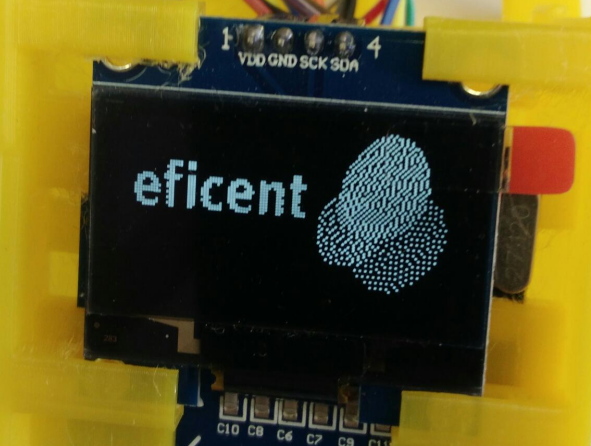
\includegraphics[width=0.7\textwidth]{images/eficent_msg.png}
	\caption[Eficent logo]{Eficent logo}
	\label{ef-logo}
\end{figure}

Then, it is time to configure the language. Hence, the \emph{idiom.json} file is read, extracting the correct idiom. A conversion id made due to some difficulties in the extraction of the language depending if it was changed the last time from the menu or from the configuration portal.

Then, after waiting for four seconds in which the Eficent logo is displayed, a welcome message is shown during other four seconds.

The result can be seen at Figure \ref{wlcm-msg}

\begin{lstlisting}[language=python]

			json_file = open('/home/pi/Raspberry_Code/idiom.json')
	        json_data = json.load(json_file)
	        json_file.close()
	        lang = json_data["language"][0]
	        print lang
	        print json_data["language"]
	        lang2 = json_data["language"]
	        if lang2 == "es":
	            lang = "es"
	        else:
	            if lang2 == "en":
	                lang = "en"
	
	        time.sleep(4)
	        welcome_msg(device,17)
	        time.sleep(4)

\end{lstlisting}

\begin{figure}[h]
	\centering
	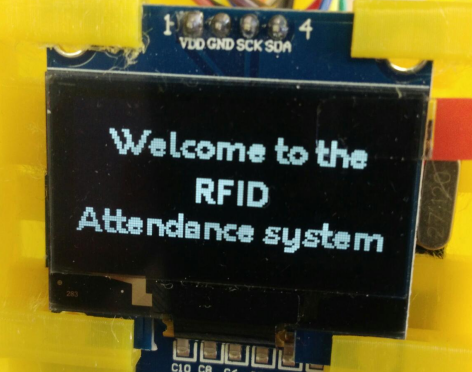
\includegraphics[width=0.7\textwidth]{images/welcome_msg.png}
	\caption[Welcome message]{Welcome message}
	\label{wlcm-msg}
\end{figure}

First, it is checked if there is WiFi connection (the function is explained later). Regarding there is connection, it is checked if the \emph{data.json} file with the different parameters does exist, because if not, it is printed a message on the screen inquiring us to go to the configuration portal (see Figure \ref{}). When the configuration file does exist, the different parameters explained before are read from it, as well as different flags values are updated (\textit{https\_on, update}). Moreover, the timezone is set so that the device clock is correctly shown.

\begin{lstlisting}[language=python]

			if have_internet():
	            while not os.path.isfile("/home/pi/Raspberry_Code/data.json"):
	                screen_drawing(device,"config1")
	                time.sleep(2)
	                screen_drawing(device,"config2")
	                time.sleep(2)
	            if os.path.isfile("/home/pi/Raspberry_Code/data.json"):
	                json_file = open('/home/pi/Raspberry_Code/data.json')
	                json_data = json.load(json_file)
	                json_file.close()
	                host = json_data["odoo_host"][0]
	                port = json_data["odoo_port"][0]
	                user_name = json_data["user_name"][0]
	                user_password = json_data["user_password"][0]
	                dbname = json_data["db"][0]
	                admin_id = json_data["admin_id"][0]
	                timezone = json_data["timezone"][0]
	                os.environ['TZ'] = tz_dic[timezone]
	                time.tzset()
	                print time.strftime('%X %x %Z')
	                if "https" not in json_data:
	                    https_on = False
	                else:
	                    https_on = True
	
	                if "update" not in json_data:
	
	                    update = False
	                else:
	                    update = True
	                print "THIS IS UPDATE: " + str(update)
	            else:
	                raise ValueError("It is not a file!")

\end{lstlisting}

\newpage
\newpage
\newpage
\pagebreak
\bibliographystyle{plain}
\bibliography{biblist}

\end{document}